% https://nymity.ch/tikz/

\documentclass[hyperref={pdfpagelabels=true},table,dvipsnames,14pt,aspectratio=169]{beamer}
\usetheme{Boadilla}

\usepackage{amsthm, amsfonts, amssymb, amsmath, graphicx}
\usepackage{amsmath}
\usepackage{amsfonts, txfonts}
\usepackage{wasysym}
\usepackage{xcolor}

\usepackage{graphicx}
\usepackage{tikz}
\usepackage{tikzpeople}
\usepackage{pgfplots}
\pgfplotsset{compat=1.15}

\pgfdeclareimage[height=5ex]{crysplogo}{crysplogo}
\pgfdeclareimage[height=5ex]{cscslogo}{cscslogo}
\pgfdeclareimage[height=5ex]{torlogo}{torlogo}
\pgfdeclareimage[height=1.5ex]{clikey}{key}
\pgfdeclareimage[height=1.5ex]{srvkey}{key-green}
\pgfdeclareimage[height=1.5ex]{clivrfkey}{key-blue}
\pgfdeclareimage[height=1.5ex]{srvvrfkey}{key-red}

\titlegraphic{
\raisebox{1ex}{
\pgfuseimage{crysplogo}~~~
\pgfuseimage{cscslogo}~~~
\pgfuseimage{torlogo}
}
}

\definecolor{AlertRed}{rgb}{1.0,0.125,0.25}
\setbeamercolor{alerted text}{fg=AlertRed}
%\setbeamerfont{alerted text}{shape=\bfseries,size=\huge}
\definecolor{auth}{RGB}{138,23,94}

\newcommand\snipdoc{
\begin{tikzpicture}[scale=.25] \draw[-,draw=black,fill=LimeGreen] (0,0) -- (2,0) -- (2,-2) -- (-1,-2) -- (-1,-1) -- cycle; \node[shape=star,star points=9,fill=auth,inner sep=0pt,star point ratio=.5,minimum size=2mm,anchor=south east] at (1.8,-1.8) {} ; \end{tikzpicture}}
\newcommand\docendive{
\begin{tikzpicture}[scale=.25] \draw[-,draw=black,fill=ForestGreen] (0,0) -- (2,0) -- (2,-11) -- (-1,-11) -- (-1,-1) -- cycle; \node[shape=star,star points=9,fill=auth,inner sep=0pt,star point ratio=.5,minimum size=2mm,anchor=south east] at (1.8,-10.8) {} ; \end{tikzpicture}}


\pgfdeclarelayer{background}
\pgfdeclarelayer{backbackground}
\pgfdeclarelayer{foreground}
\pgfsetlayers{backbackground,background,main,foreground}   %% some additional layers for demo

\usetikzlibrary{shapes,decorations.shapes}
\tikzset{>=latex}


\title{Walking Onions}
\subtitle{Scaling Anonymity Networks while Protecting Users}
\author[Chelsea Komlo]{Chelsea H. Komlo}
\institute{\small Joint work with Nick Mathewson, Ian Goldberg}
\date{\small USENIX Security, 13 August, 2020}

\begin{document}
\setbeamertemplate{itemize items}[triangle]

\begin{frame}
        \thispagestyle{empty}
        \maketitle
\end{frame}


\begin{frame}
\frametitle{Motivation}
  \begin{itemize}
    \item Design protocols that enable anonymity networks like Tor to scale
      significantly beyond their current sizes.
        \begin{itemize}
          \item Add relays to network to increase capacity
          \item While not increasing the overhead to clients to participate.
        \end{itemize}
    \item Do all of this in a way that does not change their existing security model
  \end{itemize}
\end{frame}

\begin{frame}
\frametitle{Our Contributions}
  \begin{itemize}
    \item Walking Onions, a set of protocols that allows anonymity networks
      like Tor to scale with constant-size overhead to users.
    \item Walking Onions maintains the existing security model for Tor in one
      variant, with a slight loss of forward secrecy in the other variant.
    \item Demonstrates performance improvements at networks the size of Tor
      today.
  \end{itemize}
\end{frame}

\begin{frame}
\frametitle{Outline}
  \begin{enumerate}
    \item Review of Current Tor and Performance Bottlenecks
    \item Requirements to maintain similar security
    \item Walking Onions
    \item Comparison to current Tor
      \begin{enumerate}
        \item Security
        \item Performance
      \end{enumerate}
  \end{enumerate}
\end{frame}

\begin{frame}
  \centering
  \huge
  Current Tor
\end{frame}

\begin{frame}
\frametitle{Current Tor Security Model}

Current Tor optimizes for security over scalability

  \begin{itemize}
    \item \textbf{Epistemic Attacks}
    \item \textbf{Route-Capture Attacks}
  \end{itemize}

\end{frame}

\begin{frame}
\frametitle{Current Tor Scalability}

Quadratic cost to client relative to number of relays.

\end{frame}

\begin{frame}
  \centering
  \huge
  Walking Onions
\end{frame}

\begin{frame}
\frametitle{New Data Structures}
ENDIVEs and SNIPs
\end{frame}

\begin{frame}
\frametitle{Vanilla Walking Onions}
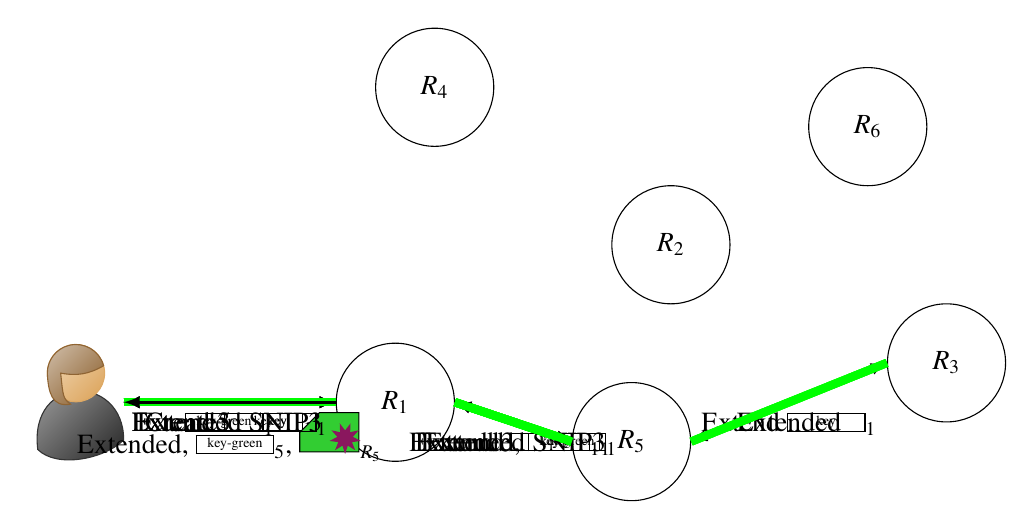
\begin{tikzpicture}
  \node[person,shirt=black,female,minimum size=1.1cm] (user1) at (3,-1) {};

  \begin{pgfonlayer}{background}

    \node[circle,draw,minimum size=1.5cm] (R1) at (7, -1) {$R_1$};
    \node[circle,draw,minimum size=1.5cm] (R2) at (10.5, 1) {$R_2$};
    \node[circle,draw,minimum size=1.5cm] (R3) at (14, -.5) {$R_3$};
    \node[circle,draw,minimum size=1.5cm] (R4) at (7.5, 3) {$R_4$};
    \node[circle,draw,minimum size=1.5cm] (R5) at (10, -1.5) {$R_5$};
    \node[circle,draw,minimum size=1.5cm] (R6) at (13, 2.5) {$R_6$};

  \end{pgfonlayer}
    \draw<1>[line width=1pt,->] (user1.east) -- (R1.west) node [below, midway]
    {Create $\pgfuseimage{clikey}_1$};

    \draw<2>[draw=green, line width=3pt,-] (user1.east) -- (R1.west) node
    [below, midway] {};
    \draw<2>[line width=1pt,->] (R1.west) -- (user1.east) node [below, midway]
    {$\pgfuseimage{srvkey}_1$};

    \draw<3>[draw=green, line width=3pt,-] (user1.east) -- (R1.west) node
    [below, midway] {};
    \draw<3>[line width=1pt,->] (user1.east) -- (R1.west) node [below, midway]
    {Extend 5 $\pgfuseimage{clikey}_1$};

    \draw<4>[draw=green, line width=3pt,-] (user1.east) -- (R1.west) node
    [below, midway] {};
    \draw<4>[line width=1pt,->] (R1.east) -- (R5.west) node [below, midway]
    {Extend $\pgfuseimage{clikey}_1$};


    \draw<5>[draw=green, line width=3pt,-] (user1.east) -- (R1.west) node
    [below, midway] {};
    \draw<5>[draw=green, line width=3pt,-] (R1.east) -- (R5.west) node {};
    \draw<5>[line width=1pt,->] (R5.west) -- (R1.east) node [below, midway]
    {Extended, $\pgfuseimage{srvkey}_1$};

    \draw<6>[draw=green, line width=3pt,-] (user1.east) -- (R1.west) node
    [below, midway] {};
    \draw<6>[draw=green, line width=3pt,-] (R1.east) -- (R5.west) node {};
    \draw<6>[line width=1pt,->] (R1.west) -- (user1.east) node [below, midway]
    {Extended, $\pgfuseimage{srvkey}_5$, $\snipdoc_{R_5}$};

    \draw<7>[draw=green, line width=3pt,-] (user1.east) -- (R1.west) node {};
    \draw<7>[draw=green, line width=3pt,-] (R1.east) -- (R5.west) node {};
    \draw<7>[line width=1pt,->] (user1.east) -- (R1.west) node [below, midway]
    {Extend 3 $\pgfuseimage{clikey}_1$};

    \draw<8>[draw=green, line width=3pt,-] (user1.east) -- (R1.west) node {};
    \draw<8>[draw=green, line width=3pt,-] (R1.east) -- (R5.west) node {};
    \draw<8>[line width=1pt,->] (R1.east) -- (R5.west) node [below, midway]
    {Extend 3 $\pgfuseimage{clikey}_1$};

    \draw<9>[draw=green, line width=3pt,-] (user1.east) -- (R1.west) node {};
    \draw<9>[draw=green, line width=3pt,-] (R1.east) -- (R5.west) node {};
    \draw<9>[line width=1pt,->] (R5.east) -- (R3.west) node [below, midway]
    {Extend $\pgfuseimage{clikey}_1$};

    \draw<10>[draw=green, line width=3pt,-] (user1.east) -- (R1.west) node {};
    \draw<10>[draw=green, line width=3pt,-] (R1.east) -- (R5.west) node {};
    \draw<10>[draw=green, line width=3pt,-] (R5.east) -- (R3.west) node {};
    \draw<10>[line width=1pt,->] (R3.west) -- (R5.east) node [below, midway]
    {Extended};

    \draw<11>[draw=green, line width=3pt,-] (user1.east) -- (R1.west) node {};
    \draw<11>[draw=green, line width=3pt,-] (R1.east) -- (R5.west) node {};
    \draw<11>[draw=green, line width=3pt,-] (R5.east) -- (R3.west) node {};
    \draw<11>[line width=1pt,->] (R5.west) -- (R1.east) node [below, midway]
    {Extended SNIP3};

    \draw<12>[draw=green, line width=3pt,-] (user1.east) -- (R1.west) node {};
    \draw<12>[draw=green, line width=3pt,-] (R1.east) -- (R5.west) node {};
    \draw<12>[draw=green, line width=3pt,-] (R5.east) -- (R3.west) node {};
    \draw<12>[line width=1pt,->] (R1.west) -- (user1.east) node [below, midway]
    {Extended SNIP3};

\end{tikzpicture}
\end{frame}

\begin{frame}
\frametitle{Telescoping Walking Onions}

\end{frame}

\begin{frame}
\frametitle{Why do these maintain Tor's existing security level?}
\end{frame}

\begin{frame}
\frametitle{}

\begin{table}[t]
\renewcommand{\arraystretch}{1.2}
\caption{Comparison: Telescoping, Single-Pass, Current Tor }

\centering
\footnotesize

\CIRCLE=achieved; \Circle=not achieved;
  \LEFTcircle=partially achieved

$\Diamond$=performance property;
  $\dagger$=security property

    \begin{tabular}{|c|c|c|c|c|}
  \hline
  & & Telescop. & Single-Pass & Current Tor \\
  \hline
  $\Diamond$ & Constant-size client download & \CIRCLE & \CIRCLE & \Circle \\
  \hline
  $\Diamond$ & One round trip per circuit built & \Circle & \CIRCLE & \Circle \\
  % Start security properties
  \hline
  $\dagger$ & \raggedright Complete client control of relays selected & \LEFTcircle & \Circle & \CIRCLE \\
  \hline
  $\dagger$ & Forward-secret relay selection& \CIRCLE & \LEFTcircle & \CIRCLE \\
  \hline
  $\dagger$ & Forward secrecy for data & \CIRCLE & \CIRCLE & \CIRCLE \\
  \hline
  $\dagger$ & \raggedright Relays unaware of their positions in paths & \LEFTcircle & \Circle & \LEFTcircle \\
  \hline
\end{tabular}

\end{table}
\end{frame}


\begin{frame}
  \centering
  \huge
  Performance Evaluation
\end{frame}

\begin{frame}
\frametitle{Simulation}
Simulation description
\end{frame}

\begin{frame}
\frametitle{Bandwidth}
\end{frame}

\begin{frame}
\frametitle{CPU}
\end{frame}

\begin{frame}
\frametitle{Summary}
\end{frame}
\end{document}
